\documentclass[a4paper,11pt,oneside]{book}

% PACCHETTI
\usepackage{hyperref}           % hyperlinks
\usepackage{tabto}              % strumento per inserire tab nel testo
\usepackage[                    % geometria della pagina
    a4paper,
    inner=2cm,
    outer=3cm,
    top=3cm,
    bottom=3cm,
    bindingoffset=1.2cm,
    headheight=14pt
]{geometry}
\usepackage[utf8]{inputenc}     % 3 pacchetti per l'italiano
\usepackage[italian]{babel}
\usepackage[T1]{fontenc}
\usepackage{titlesec}           % custom chapter titles

\usepackage{fancyhdr}
\usepackage{multicol}
\usepackage[arrowdel]{physics} 
\usepackage{amsmath}
\usepackage{tikz}

\usepackage{graphicx}           % IMMAGINI
\graphicspath{ {./images/} }
\usepackage{wrapfig}

\usepackage{csquotes}
\usepackage{caption}

% INFORMAZIONI SUL DOCUMENTO
\title{\Large{\textbf{Fisica 1}}}
\author{Enrico Bragastini}
\titleformat{\chapter}[display]{\normalfont\bfseries}{}{0pt}{\LARGE}


% CONTENUTO
\begin{document}
\pagestyle{fancy}
\fancyhf{}
\rhead{}
\lhead{\nouppercase\leftmark}
\cfoot{\thepage}
\frontmatter

% Prima pagina - Titolo
\maketitle
\tableofcontents

\mainmatter
\chapter{Nozioni di base}
\section{Misura di una grandezza}
Una \textbf{grandezza fisica} è la proprietà di un fenomeno, corpo o sostanza, che può essere espressa
quantitativamente mediante un numero e un riferimento.

\noindent La misura di una grandezza può avvenire con due modalità:
\begin{itemize}
    \item Mediante un dispositivo sperimentale
    \item Confronto con un'altra grandezza omogenea di riferimento e costante
\end{itemize}

\noindent L'espressione di una grandezza fisica avviene nella forma:
\begin{equation*}
    \text{Numero} + \text{\underline{\emph{Unità di misura}}}
\end{equation*}

\section{Grandezze fisiche fondamentali e derivate}
Possiamo distinguere le grandezze fisiche in \underline{fondamentali} e \underline{derivate}.

\noindent Le \textbf{grandezze fisiche fondamentali} sono:
\begin{itemize}
    \item Lunghezza                 \tabto{7cm} [L]
    \item Massa                     \tabto{7cm}  [M]
    \item Tempo                     \tabto{7cm}  [t]
    \item Intensità Di Corrente     \tabto{7cm}  [i]
    \item Temperatura Assoluta      \tabto{7cm}  [T]
\end{itemize}

\noindent Le \textbf{grandezze fisiche derivate} sono grandezze che possono essere
espresse in forma di combinazioni matematiche delle grandezze fondamentali.
Alcuni esempi di grandezze derivate sono:
\begin{itemize}
    \begin{multicols}{2}
        \item Superficie
        \item Volume
        \item Velocità
        \item Accelerazione
        \item Forza
        \item Pressione
    \end{multicols}
\end{itemize}

\section{Sistemi di Unità di Misura}
\begin{center}
    \bgroup
    \def\arraystretch{1.5}
    \begin{tabular}{ |c| c c c c c|}
        \hline
        SISTEMA     & Lunghezza & Massa & Tempo & Corrente & Temperatura \\
        \hline
        MKS (s. i.) & m         & kg    & s     & A        & °K          \\
        \hline
        cgs         & cm        & g     & s     & A        & °K          \\
        \hline
    \end{tabular}
    \egroup
\end{center}

\subsection{Ulteriori Unità di Misura}
Esistono ulteriori sistemi di unità di misura che permettono di avere maggiore comodità
nelle misurazioni di particolari grandezze.
Se ne elencano alcuni:

\begin{enumerate}
    \item Lunghezza:    \tabto{3cm} Ångströms, Anno-Luce
    \item Tempo:        \tabto{3cm} Minuto, Ora
    \item Volume:       \tabto{3cm} Litro
    \item Velocità:     \tabto{3cm} Chilometro/Ora
    \item Pressione:    \tabto{3cm} Atmosfera, Millimetro di mercurio
    \item Energia:      \tabto{3cm} Elettrovolt, Chilovattora
\end{enumerate}

\section{Notazione Scientifica}
Per i numeri particolarmente grandi o piccoli risulta comodo rappresentarli
in \textbf{Notazione Scientifica} utilizzando le potenze del 10.

La notazione scientifica permette di scrivere un numero in cui compare una sequenza molto lunga di zeri in forma compatta.
In matematica si dice che un numero è scritto in notazione scientifica se è della forma $n\cdot10^e$

~\newline
\underline{Esempio:}
\begin{equation*}
    1,2 \cdot 10^5
\end{equation*}
Un numero in \emph{notazione scientifica} è quindi composto da:
\begin{itemize}
    \item Un numero compreso n tale che $1 \leq n < 10$
    \item Una potenza del 10 con esponente intero
\end{itemize}

\newpage
\section{Analisi Dimensionale}
Quando si è di fronte ad una formula fisica o si svolgono calcoli con grandezze fisiche e unità di misura,
per verificare la plausibilità della formula data e la consistenza
dei calcoli svolti si può ricorrere all'analisi dimensionale.

Eseguire l'analisi dimensionale di una formula, o più in generale di un'equazione fisica,
vuol dire ricavare le dimensioni di ognuno dei due membri allo scopo di verificare che esse coincidano:
se così non fosse ci sarebbe necessariamente qualcosa di sbagliato, perché avremmo a che fare con un'equazione
dimensionalmente non consistente.


\section{Sistemi di Coordinate}
Molti aspetti della fisica hanno in qualche modo a che fare con la descrizione di un punto dello spazio.
Ad esempio, la descrizione matematica del moto di un corpo richiede un metodo che descriva la successione
delle posizioni occupate dal corpo nel tempo.

\subsection{Coordinate cartesiane}
In due dimensioni questa descrizione può essere realizzata con l’uso di un sistema di \textbf{coordinate cartesiane}
in cui due assi perpendicolari si intersecano in un punto definito come punto origine.
Le coordinate cartesiane sono anche dette \emph{coordinate rettangolari}.
\begin{figure}[h]
    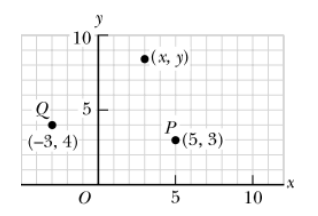
\includegraphics[scale=0.5]{coordinate_cartesiane}
    \centering
\end{figure}

\subsection{Coordinate scalari}
Talvolta è più conveniente rappresentare un punto in un piano tramite le sue \textbf{coordinate polari piane} $(r, \theta)$.

\begin{figure}[h]
    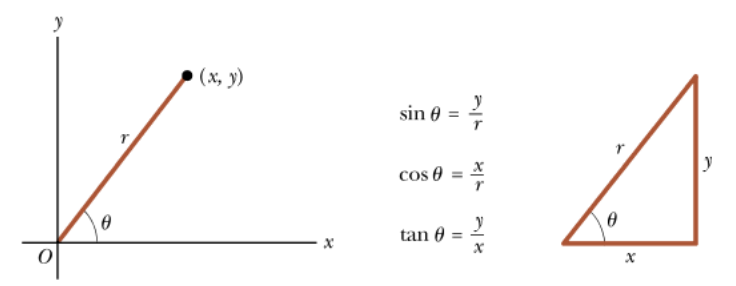
\includegraphics[scale=0.5]{coordinate_polari}
    \centering
\end{figure}
In questo sistema di coordinate polari, r è la distanza dall’origine al punto di coordinate
cartesiane $(x, y)$ e $\theta$ è l’angolo fra un asse fisso e la semiretta tracciata dall’origine al punto, generalmente
misurato in verso antiorario dall’asse x positivo.

\paragraph{Conversione delle coordinate} Partendo dalle coordinate polari, si possono ottenere le coordinate cartesiane
tramite le seguenti equazioni:
\begin{itemize}
    \item $x = r \cdot \cos{\theta}$
    \item $y = r \cdot \sin{\theta}$
\end{itemize}
Inoltre, sfruttando la trigonometria si possono ottenere queste altre informazioni:
\begin{itemize}
    \item $\tan{\theta} = \frac{y}{x}$
    \item $r = \sqrt{x^2 + y^2}$
\end{itemize}

\section{Grandezze scalari e grandezze vettoriali}

\subsection{Grandezza scalare}
Una \emph{grandezza scalare} è una grandezza che è specificata solamente da un valore con una certa unità di misura e non associata con una direzione.

Alcune grandezze scalari sono \emph{sempre positive}, come la massa e la velocità scalare.
Altre, come la temperatura, possono avere valori \emph{sia positivi che negativi}.
Per manipolare le quantità scalari si adoperano le \textbf{normali regole dell’aritmetica}.

\subsection{Grandezza vettoriale}
Una grandezza vettoriale è una grandezza che, per essere specificata,
ha bisogno sia di un numero con le sue unità di misura (\textbf{modulo del vettore}), sia di una \textbf{direzione orientata}.

Per rappresentare un vettore, si utilizza una lettera sormontata da una freccia come da esempio:
\begin{equation*}
    \vec{A}
\end{equation*}

\newpage
\section{Proprietà e operazioni con i vettori}
\subsection{Uguaglianza di due vettori}
Due vettori $\vec{A}$ e $\vec{B}$ sono \textbf{uguali} se sono uguali i loro \emph{moduli}, la \emph{direzione} e il \emph{verso}.
L'uguaglianza è \emph{indipendente dall'origine}, ovvero i vettori possono essere traslati sul grafico in base alla necessità
senza che venga persa la loro uguaglianza.
\begin{figure}[h]
    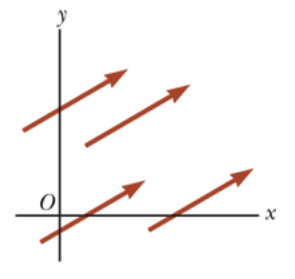
\includegraphics[scale=0.5]{uguaglianza_vettori}
    \centering
\end{figure}

\subsection{Somma tra vettori (metodo grafico)}
La somma tra vettori può essere svolta rapidamente in modo grafico.

In generale, se si vogliono sommare due spostamenti rappresentati dai due vettori $\vec{a}$ e $\vec{b}$ come di seguito rappresentato:
\begin{figure}[h]
    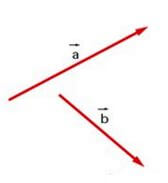
\includegraphics[scale=0.5]{vettori_da_sommare}
    \centering
\end{figure}

\paragraph{Metodo punta-coda:} Spostiamo uno dei due vettori in modo tale che la sua coda coincida con la punta del primo vettore.

~\newline
\noindent Riferendoci al nostro caso, spostiamo il vettore $\vec{b}$ vettore in modo tale che la sua coda coincida con la
punta del vettore $\vec{a}$, come di seguito rappresentato:
\begin{figure}[h]
    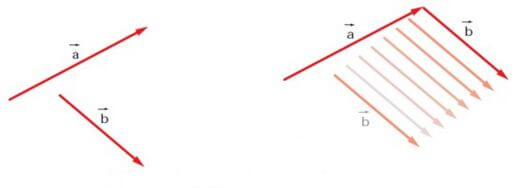
\includegraphics[scale=0.5]{punta_coda}
    \centering
\end{figure}

Come è possibile notare dalla figura precedente lo spostamento del vettore $\vec{b}$ deve essere effettuato in modo
tale che la freccia rimanga sempre parallela a se stessa.
Lo spostamento totale si ottiene unendo la coda del vettore $\vec{a}$ con la punta del vettore $\vec{a}$, come di seguito
rappresentato:
\begin{figure}[h]
    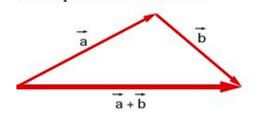
\includegraphics[scale=0.5]{vettori_sommati}
    \centering
\end{figure}

Si noti che in generale il modulo del vettore somma non è uguale alla somma dei moduli dei singoli spostamenti.

\subsection{Opposto di un vettore}
L'\textbf{opposto di un vettore} $\vec{A}$ è definito come il vettore che sommato a $\vec{A}$ permette di ottenere 0.
\begin{equation*}
    \vec{A} + (- \vec{A} ) = 0
\end{equation*}
Il vettore $(-\vec{A})$ è quindi un vettore che ha lo \textbf{stesso modulo} di $\vec{A}$, con la \textbf{stessa direzione} ma di \textbf{verso opposto}.

\subsection{Sottrazione tra vettori}
La \textbf{sottrazione tra vettori} si ottiene sfruttando la definizione di \emph{vettore opposto}.
Quindi, si vuole sottrarre il vettore $\vec{B}$ al vettore $\vec{A}$, basta \emph{sommarne l'opposto}.
\begin{equation*}
    \vec{A} - \vec{B} = \vec{A} + (- \vec{B})
\end{equation*}

\subsection{Prodotto tra un vettore e uno scalare}
\begin{itemize}
    \item Se un vettore $\vec{A}$ viene moltiplicato per una quantità scalare positiva $m$,
          allora il prodotto è $m\vec{A}$ e possiede la stessa direzione di A e modulo $mA$.
    \item Se un vettore $\vec{A}$ viene moltiplicato per una quantità scalare negativa $-m$,
          allora il prodotto è $-m\vec{A}$ e possiede direzione opposta di A e modulo $mA$.
\end{itemize}

\newpage
\section{Componenti di un vettore e vettori unitari}
\subsection{Componenti di un vettore}
Il metodo geometrico di somma vettoriale non è raccomandabile in quelle situazioni in cui si richiede una precisione elevata, oppure nei problemi in tre dimensioni.
Esiste un metodo per sommare i vettori che fa uso delle \emph{proiezioni dei vettori} lungo gli assi coordinati.
Queste proiezioni sono chiamate \textbf{componenti del vettore} o anche componenti rettangolari del vettore. Un vettore può essere descritto in modo completo dai suoi componenti.

Un vettore $\vec{A}$ può essere espresso come come \emph{somma di due vettori componenti}: $\vec{A_x}$, parallelo all'asse $x$, sommato a $\vec{A_y}$,
parallelo all'asse $y$.
\begin{figure}[h]
    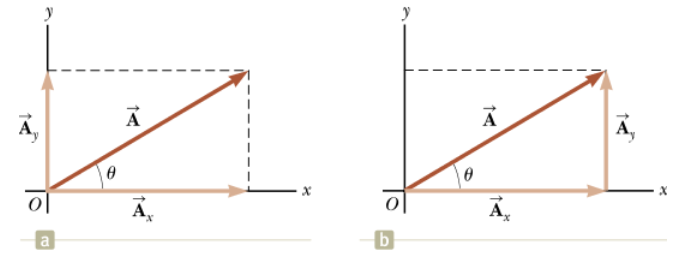
\includegraphics[scale=0.5]{vettori_componenti}
    \centering
\end{figure}

\noindent Si ottengono quindi le seguenti relazioni:
\begin{itemize}
    \item $\vec{A} = \vec{A_x} + \vec{A_y}$
    \item $\vec{A_x} = A \cos{\theta}$
    \item $\vec{A_y} = A \sin{\theta}$
    \item $A = \sqrt{A_x^2 + A_y^2}$
    \item $\theta = \tan[-1](\frac{A_y}{A_x})$
\end{itemize}
Nell’affrontare un problema fisico si può scegliere di specificare un vettore $\vec{A}$
per mezzo delle sue componenti $\vec{A_x}$ e $\vec{A_y}$ oppure per mezzo del suo modulo A e dell’angolo $\theta$.

\subsection{Vettori unitari}
Un \textbf{vettore unitario} è un \emph{vettore adimensionale} il cui modulo è esattamente 1.
I vettori unitari hanno l'unico scopo di indicare una direzione orientata e non hanno nessun altro significato fisico.
Il modulo dei vettori unitari è uguale a 1, ovvero $\abs*{\hat{i}} = \abs*{\hat{j}} = \abs*{\hat{k}} = 1$

Useremo i simboli $\hat{i}$, $\hat{j}$, e $\hat{k}$ per rappresentare i vettori unitari che puntano rispettivamente nelle direzioni positive x, y e z.

\newpage
\begin{figure}[h]
    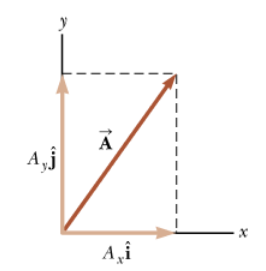
\includegraphics[scale=0.5]{vettori_unitari}
    \centering
\end{figure}
Consideriamo un vettore $\vec{A}$ che giace nel piano $xy$ come in figura.
Il prodotto della componente $A_x$ per il vettore unitario $\hat{i}$ è il vettore $\vec{A_x} = A_x \hat{i}$ parallelo all'asse delle $x$ e di modulo $\abs{A_x}$.
Analogamente, $\vec{A_y} = A_y \hat{j}$ è un vettore di modulo $\abs{A_y}$ parallelo all’asse $y$.
Così, nella notazione dei vettori unitari, il vettore $\vec{A}$ è
\begin{equation*}
    \vec{A} = A_x \hat{i} \cdot A_y \hat{j}
\end{equation*}

\subsection{Somma tra vettori (metodo con vettori unitari)}
Quando il metodo grafico non risulta sufficientemente accurato ci si può avvalere dell'utilizzo delle componenti dei vettori da sommare.

Si supponga di voler sommare il vettore $\vec{A}$ composto da $\vec{A_x}$ e da $\vec{A_y}$ al vettore $\vec{B}$
composto da $\vec{B_x}$ e da $\vec{B_y}$.

\begin{figure}[h]
    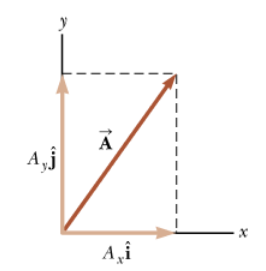
\includegraphics[scale=0.5]{vettori_unitari}
    \centering
\end{figure}

\noindent Per effettuare questa somma basta sommare separatamente le componenti $x$ e $y$. Il vettore risultante $\vec{R} = \vec{A} + \vec{B}$
si ottiene con:
\begin{equation*}
    \vec{R} = (A_x \hat{i} + A_y \hat{j}) + (B_x \hat{i} + B_y \hat{j})
\end{equation*}
ovvero
\begin{equation*}
    \vec{R} = (A_x+ B_x) \hat{i} + (A_y + B_y) \hat{j}
\end{equation*}

~\newline
\noindent Il vettore ottenuto può essere a sua volta visto come $\vec{R} = R_x \hat{i} + R_y \hat{j}$.



\chapter{Cinematica}

La \textbf{Cinematica} è un ramo della \textbf{meccanica classica} che si occupa di descrivere quantitativamente il moto dei corpi, indipendentemente dalle cause del moto stesso.

\section{Moto in una dimensione}

\paragraph{Punto materiale}
Nello studio del moto traslatorio utilizziamo il modello \textbf{punto materiale} e descriviamo il moto di un corpo approssimandolo ad
“una particella” senza considerare le sue dimensioni reali.

In generale un punto materiale è quel corpo che \emph{ha una massa} ma \emph{ha dimensioni infinitesimali}.

\section{Posizione, spostamento e distanza}

\paragraph{Posizione} Indichiamo come posizione il punto occupato \emph{istante per istante} dal punto materiale oggetto di studio.
Un corpo è considerato \emph{in moto} se la sua posizione cambia con il passare del tempo.

\paragraph{Spostamento} Lo spostamento, indicato con $\Delta x$\footnote{La lettera greca $\Delta$ indica in generale una \emph{variazione}} è definito come la variazione della sua posizione in un certo intervallo di tempo.

Se da $x_i$ il punto materiale raggiunge la posizione $x_f$ il suo spostamento è definito come la posizione finale meno la posizione iniziale:
\begin{equation*}
    \Delta x = x_f - x_i
\end{equation*}
Lo spostamento è una \emph{grandeza vettoriale}, ma sul moto rettilineo è possibile considerarlo come una \emph{lunghezza scalare}.

\paragraph{Distanza percorsa}
La distanza percorsa \emph{non è lo spostamento}. La distanza indica la lunghezza del cammino percorso da una particella.

Supponiamo che un'automobile parta dal punto $A$, arrivi al punto $B$ e poi ritorni al punto $A$. In questo caso abbiamo che lo spostamento
è nullo, infatti $x_i = x_f$, ovvero $\Delta x = 0$. Mentre la distanza percorsa corrisponde a $2 (B-A)$.

\section{Velocità media e istantanea}

\paragraph{Velocità media}
La \textbf{velocità media}, $v_{m}$ di un punto materiale, è definita come il rapporto tra lo spostamento $\Delta x$ del punto materiale
e l’intervallo di tempo $\Delta t$ durante il quale lo spostamento è avvenuto:
\begin{equation*}
    v_{x,media} \equiv \frac{\Delta x}{\Delta t}
\end{equation*}

\begin{itemize}
    \item L'unità di misura è: $\frac{m}{s}$
    \item Se $\Delta x > 0$ (spostamento nel verso positivo), allora $v_m > 0$.
    \item Se $\Delta x < 0$ (spostamento nel verso negativo), allora $v_m < 0$
\end{itemize}

\paragraph{Velocità media scalare}
La velocità scalare media $v_{media}$ di un punto materiale, una quantità scalare, è definita come il rapporto
fra la distanza totale $d$ percorsa e l’intervallo di tempo impiegato a percorrerla:
\begin{equation*}
    v_{m} \equiv \frac{d}{\Delta t}
\end{equation*}

\paragraph{Velocità istantanea}
La velocità istantanea $v_x$ di un corpo in un determinato istante di tempo $t$ è uguale al valore limite del rapporto $\frac{\Delta x}{\Delta t}$
quando $\Delta t$ tende a $0$. Nel linguaggio del calcolo differenziale questo limite è la derivata di x rispetto a t:
\begin{equation*}
    v_x \equiv \lim_{\Delta t \to 0} \frac{\Delta x}{\Delta t} = \frac{dx}{dt}
\end{equation*}

~\newline
\underline{Esempio:} \newline
Espressione analitica dello spostamento di un punto materiale: $x=-4t + 2t^2$
Calcolo della velocità istantanea a $t = 2,5s$
\begin{align*}
    x             & = -4t + 2t^2 \\
    \frac{dx}{dt} & = -4 + 4t    \\
    v_x           & = 6 \; m/s
\end{align*}

\section{Moto Rettilineo Uniforme}
Un corpo si muove con \textbf{moto rettilineo uniforme} quando si sposta lungo una retta con velocità costante.

Basandoci su questa definizione si possono ricavare le seguenti equazioni:
\begin{itemize}
    \item $v_x = \text{costante}$
    \item $v_{x,media} = v_x$
    \item $v_x = \frac{\Delta x}{\Delta t} = \frac{x_f - x_i}{t_f - t_i}$
    \item $x_f = x_i + \frac{v_x(t_f - t_i)}{v_x \Delta t}$, scegliendo \tiny $\begin{aligned} t_i&=0 \\ t_f&=t \end{aligned}$ \normalsize otteniamo $x_f = x_i + v_x \cdot t$
\end{itemize}

\section{Accelerazione media e istantanea}

\paragraph{Accelerazione media} Quando la velocità cambia nel tempo, si dice che la particella sta accelerando.
L’accelerazione media $a_{x,media}$ del punto materiale è definita come la variazione della velocità
$\Delta v_x$ divisa per l’intervallo di tempo $\Delta t$ in cui avviene la variazione:
\begin{equation*}
    a_{x,media} \equiv \frac{\Delta v_x}{\Delta t} = \frac{v_{xf} - v_{xi}}{t_f - t_i   }
\end{equation*}
L'unità di misura dell'accelerazione è $m/s^2$

\paragraph{Accelerazione instantanea} Si definisce l'accelerazione istantanea come il limite dell'accelerazione
media quando $\Delta t$ tende a zero.
\begin{equation*}
    a_{x,media} \equiv \lim_{\Delta t \to 0} \frac{\Delta v_x}{\Delta t} = \frac{dv_x}{dt} = \frac{d}{dt} (\frac{dx}{dt}) = \frac{d^2x}{dt^2}
\end{equation*}
L’accelerazione istantanea è la derivata della velocità rispetto al tempo che è anche la pendenza della curva del grafico velocità–tempo.

\section{Moto rettilineo uniformemente accelerato}
Nel caso del \textbf{moto rettilineo uniformemente accelerato}, il moto del \emph{punto materiale} avviene con \emph{accelerazione costante}.

~\newline
\noindent Se il moto avviene con accelerazione costante, allora la velocità media e la velocità istantanea coincidono.
\begin{equation*}
    a_x = \frac{v_{xf}-v_{xi}}{t_f-t_i}
\end{equation*}
Supponendo $t_i = 0$ otteniamo $a_x = \frac{v_{xf}-v_{xi}}{t}$ e quindi $v_{xf} = v_{xi} + a_x t$ (per $a_x$ costante)

Poiché la velocità varia linearmente con il tempo, la velocità media in un intervallo di tempo
arbitrario è uguale alla \emph{media aritmetica} della velocità iniziale $v_{xi}$ e della velocità finale $v_{xf}$:
\begin{equation*}
    v_{media} = \frac{v_{xi} + v_{xf}}{2} = \frac{1}{2} (v_{xi} + v_{xf}) \; \; \text{(per } a_{x} \text{ costante)}
\end{equation*}

Ora, ricordando che $\Delta x = x_f - x_i$ e che $\Delta t = t_f - 0 = t$, si ottiene:
\begin{equation*}
    x_f - x_i = v_{media} t = \frac{1}{2} (v_{xi} + v_{xf}) t
\end{equation*}
\begin{align*}
    x_f & = x_i + \frac{1}{2} (v_{xi} + v_{xf}) t                                         \\
    x_f & = x_i + \frac{1}{2} [v_{xi} + (v_{xi} + a_x t)] t                               \\
    x_f & = x_i + v_{xi} t + \frac{1}{2} a_x t^2 \; \; \text{(per } a_x \text{ costante)}
\end{align*}
Si può infine ottenere un’espressione per la velocità finale che non contiene il tempo:
\begin{equation*}
    v_{xf}^2 = v_{xi}^2 + 2ax(x_f - x_i)
\end{equation*}

\subsection{Corpi in caduta libera}
È un fatto ben noto che vicino alla superficie della Terra e senza la resistenza dell’aria,
tutti i corpi sotto l’influenza della gravità terrestre cadono verso la Terra con la \textbf{stessa accelerazione costante}.

Indicheremo il modulo dell’accelerazione di caduta libera, detta anche accelerazione di gravità con il simbolo $g$.
Sulla superficie della Terra, il valore di $g$ è approssimativamente 9.80 $m/s^2$.

\section{Moto in due dimensioni}
A differenza del moto in una sola dimensione, nel \emph{moto a due dimensioni}, le posizioni di inizio e di fine dello spostamento
di un punto materiale sono \textbf{grandezze vettoriali} e sono indicate da $\vec{r_i}$ e $\vec{r_f}$.

La posizione è quindi descritta dal \emph{vettore} $\vec{r}$. Lo spostamento del punto materiale è indicato con $\Delta \vec{r} = \vec{r_f}-\vec{r_i}$.

\paragraph{Velocità media}
La velocità media è definita come:
\begin{equation*}
    \vec{v}_{media} \equiv \frac{\Delta \vec{r}}{\Delta t}
\end{equation*}
La direzione e il verso di $\vec{v}_{media}$ sono le stesse di $\Delta \vec{r}$ in quanto $\Delta t$ è uno scalare.

\paragraph{Velocità istantanea}
La velocità istantanea è definita come:
\begin{equation*}
    \vec{v} \equiv \lim_{\Delta t \to 0} \frac{\Delta \vec{r}}{\Delta t} = \frac{d \vec{r}}{dt}
\end{equation*}
La velocità istantanea è la \emph{derivata} del vettore posizione rispetto al
tempo. La direzione del vettore velocità istantanea in un punto è quella della retta tangente alla traiettoria in quel punto ed è orientata nel verso del moto.

\paragraph{Accelerazione media}
Conoscendo la velocità in ciascuno dei due punti è possibile determinare l'accelerazione media:
\begin{equation*}
    \vec{a}_{media} \equiv \frac{\Delta \vec{v}}{\Delta t} = \frac{\vec{v_f} - \vec{v_i}}{t_f - t_i}
\end{equation*}

\paragraph{Accelerazione istantanea}
Dall'accelerazione media è possibile ricavare l'accelerazione istantanea:
\begin{equation*}
    \vec{a} \equiv \lim_{\Delta t \to 0} \frac{\Delta \vec{v}}{\Delta t} = \frac{d\vec{v}}{dt}
\end{equation*}

\newpage
\subsection{Moto in due dimensioni con accelerazione costante}
Il moto in due dimensioni può essere modellizzato come \emph{due moti indipendenti} lungo
ciascuna delle due direzioni ortogonali che possono essere associate agli \emph{assi $x$ e $y$}.
Qualunque azione in direzione $x$ non influenza il moto in direzione $y$ e viceversa.

\begin{figure}[h]
    \centering
    \begin{tikzpicture}
        \draw[thin,gray!40] (0,0) grid (4,4);
        \draw[<->] (0,0)--(4,0) node[right]{$x$};
        \draw[<->] (0,0)--(0,4) node[above]{$y$};
        \draw[line width=2pt,black,-stealth](0,0)--(2.5,2.5) node[anchor=south west]{$P(x,y)$};
        \draw[line width=1pt,black,-stealth](0,0)--(0,2.5) node[anchor=north east]{$y \hat{j}$};
        \draw[line width=1pt,black,-stealth](0,0)--(2.5,0) node[anchor=north east]{$x \hat{i}$};

        \draw[dashed,line width=0.5pt,black,](0,2.5)--(2.5,2.5);
        \draw[dashed,line width=0.5pt,black,](2.5,0)--(2.5,2.5);
    \end{tikzpicture}
\end{figure}
\noindent Il \textbf{vettore posizione} per un punto materiale che si muove nel piano $xy$ può essere scritto come
\begin{equation*}
    \vec{r} = x\hat{i} + y\hat{j}
\end{equation*}
Se il vettore posizione è noto, la \textbf{velocità} può essere ricavata:
\begin{equation*}
    \vec{v} = \frac{d\vec{r}}{dt} = \frac{dx}{dt}\hat{i}+\frac{dy}{dt}\hat{j} = v_x \hat{i} + v_y \hat{j}
\end{equation*}
Essendo l'\textbf{accelerazione costante}, anche $a_x$ e $a_y$ sono costanti.

\noindent Sostituendo $v_{xf} = v_{xi} + a_x t$ e $v_{yf} = v_{yi} + a_y t$ alla formula della velocità si ottiene:
\begin{align*}
    v_f & = (v_{xi} + a_x t)\hat{i} + (v_{yi} + a_y t)\hat{j}            \\
        & = (v_{xi}\hat{i} + v_{yi}\hat{j}) + (a_x\hat{i} + a_y\hat{j})t \\
        & = v_i + at
\end{align*}

\noindent Analogamente le coordinate $x_f$ e $y_f$ sono date da:
\begin{align*}
    x_f & = x_i + v_{xi}t + \frac{1}{2}a_xt^2 & y_f & = v_i + v_{yi} + \frac{1}{2}a_yt^2
\end{align*}

\noindent Sostituendole nella formula del vettore posizione si ottiene:
\begin{align*}
    \vec{r}_f & = x\hat{i} + y\hat{j}                                                                                            \\
              & = (x_i + v_{xi}t + \frac{1}{2}a_xt^2)\hat{i} + (v_i + v_{yi} + \frac{1}{2}a_yt^2)\hat{j}                         \\
              & = (x_i \hat{i} + y_i \hat{j}) + (v_{xi} \hat{i} + v_{yi} \hat{j})t + \frac{1}{2} (a_x \hat{i} + a_y \hat{j}) t^2 \\
              & = \vec{r}_i + \vec{v}_i t + \frac{1}{2} \vec{a} t^2
\end{align*}

\subsection{Moto dei proiettili}
Il moto dei proiettili (moto parabolico) può essere analizzato mediante due ipotesi:
\begin{enumerate}
    \item l’accelerazione di caduta libera si mantiene costante per tutto il moto ed è diretta verso il basso
    \item l’effetto della resistenza dell’aria è trascurabile
\end{enumerate}
Sotto queste ipotesi, la traiettoria del proiettile è \emph{sempre una parabola}.

\begin{figure*}[h]
    \centering
    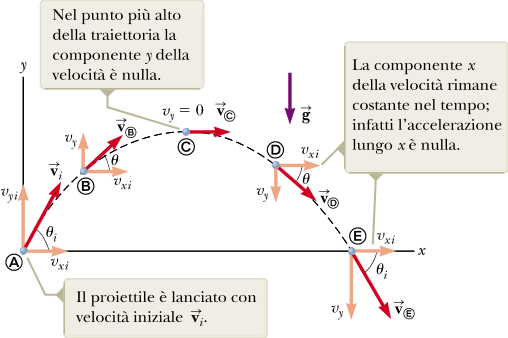
\includegraphics[scale=0.5]{moto_proiettili}
\end{figure*}

Il moto del proiettile è considerabile con accelerazione orizzontale $a_x = 0$,
mentre l'accelerazione verticale è costante: $\vec{a} = \vec{g}$. L'espressione del vettore posizione del proiettile è quindi pari a:
\begin{equation*}
    \vec{r}_f = \vec{r}_i + \vec{v}_i t + \frac{1}{2} \vec{g}t^2
\end{equation*}
dove le due componenti di $\vec{v}_i$ sono:
\begin{align*}
    v_{xi} & = v_i \cos{\theta_i} & v_{yi} & = v_i \sin{\theta_i}
\end{align*}

Tenendo a mente che il moto del proiettile è la sovrapposizione di un punto materiale con velocità orizzontale costante
\begin{equation*}
    x_f = x_i + v_{xi}t
\end{equation*}
e un punto materiale
con accelerazione verticale costante ($a_y = -g$), otteniamo le seguenti relazioni:
\begin{itemize}
    \item $v_{yf} = v_{yi} - gt$
    \item $v_{y,media} = \frac{v_{yi} + v_{yf}}{2}$
    \item $y_f = y_i + \frac{1}{2} (v_{yi} + v_{yf})t$
    \item $y_f = y_i + v_{yi}t - \frac{1}{2} gt$
    \item $v_{yf}^2 = v_{yi}^2 -2g(y_f - y_i)$
\end{itemize}

\paragraph{Altezza massima}
L'altezza massima $h_{max}$ raggiunta dal corpo lanciato è determinabile notando che nel \emph{picco} la velocità verticale si annulla $v_y = 0$
\begin{equation*}
    v_{yf} = v_{yi} - gt \; \rightarrow \; 0 = v_i \sin{\theta_i} -gt
\end{equation*}
\begin{equation*}
    t = \frac{v_i \sin{\theta_i}}{g} \;\;\; \text{(tempo per raggiungere } h_{max} \text{)}
\end{equation*}
Possiamo utilizzare questa espressione del tempo per calcolare l'altezza massima raggiunta. Partendo dalla precedente espressione per il calcolo di
$y_f$ si sostituisce t con l'espressione appena trovata e $y_f$ diventa l'altezza $h_{max}$
\begin{align*}
    y_f = y_i + v_{yi}t - \tfrac{1}{2}gt^2 \;\; \rightarrow \;\; h_{max} & = 0 + (v_i \sin{\theta_i})\tfrac{v_i \sin{\theta_i}}{g} - \tfrac{1}{2}g(\tfrac{v_i \sin{\theta_i}}{g})^2 \\
    h_{max}                                                              & = \frac{v_i^2 \sin^2{\theta_i}}{2g}
\end{align*}

\paragraph{Gittata}
La gittata $R$ è la distanza orizzontale percorsa dal proiettile in un \emph{tempo doppio} di quello necessario a raggiungere l'altezza massima.
\begin{align*}
    x_f & = x_i + v_{xi}t                 & R & = v_{xi}t = (v_i \cos{\theta_i})2t                                                                     \\
    t   & = \tfrac{v_i \sin{\theta_i}}{g} & R & = (v_i \cos{\theta_i}) \tfrac{2v_i \sin{\theta_i}}{g} = \tfrac{2v_i^2 \sin{\theta_i}\cos{\theta_i}}{g}
\end{align*}
Poiché vale la relazione $2\sin{\theta_i}\cos{\theta_i} = \sin{2\theta}$, si può scrivere:
\begin{equation*}
    R = \frac{v_i^2 \sin{2\theta_i}}{g}
\end{equation*}


\section{Moto Circolare Uniforme}
Il \emph{moto circolare} è uno dei moti semplici studiati dalla fisica e dalla cinematica, e consiste in un moto di un punto materiale lungo una circonferenza. 

Se il \textbf{moto circolare} è \textbf{uniforme} significa che \textbf{è costante il vettore velocità angolare}, cioè si ha \textbf{velocità lineare costante in modulo}. 
Poiché comune in molte situazioni fisiche, questo tipo di moto viene schematizzato in un modello di analisi, detto \textbf{punto materiale in moto circolare uniforme}.

Il \textbf{vettore velocità}, che è sempre \textbf{tangente alla traiettoria}, è \textbf{perpendicolare al raggio} della traiettoria circolare. Quindi la direzione del vettore velocità cambia continuamente.

In un moto circolare uniforme il \textbf{vettore accelerazione} può avere solamente un componente \textbf{perpendicolare alla traiettoria}, ovvero \emph{diretto verso il centro della circonferenza}.
\begin{figure*}[h]
    \centering
    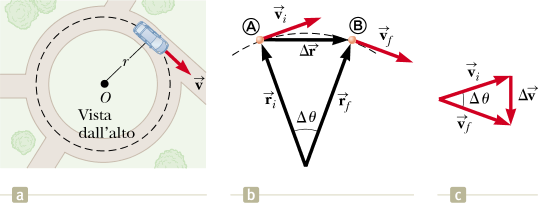
\includegraphics[scale=0.5]{moto_circolare_uniforme}    
\end{figure*}

\paragraph{Accelerazione media}
Partendo dall'equazione $\vec{a}_{media} = \tfrac{\Delta \vec{v}}{\Delta t}$ e conoscendo la relazione tra le lunghezze nei due triangoli delle figure
\begin{equation*}
    \tfrac{\abs{\Delta \vec{v}}}{v} = \tfrac{\abs{\Delta \vec{r}}}{r}
\end{equation*}
è possibile calcolare il modulo dell'accelerazione media nell'intervallo di tempo in cui avviene lo spostamento:
\begin{equation*}
    \abs{\vec{a}_{media}} = \frac{\abs{\Delta \vec{v}}}{\abs{\Delta t}} = \frac{v}{r}\frac{\abs{\Delta \vec{r}}}{\Delta t}
\end{equation*}
Infine, passando al limite per $\Delta t \to 0$, si ottiene per il modulo dell'accelerazione:
\begin{equation*}
    a_c = \frac{v^2}{r}
\end{equation*}
Questo tipo di accelerazione è chiamata \textbf{accelerazione centripeta}.

\paragraph{Periodo}
È conveniente descrivere il moto circolare uniforme di un punto materiale su una circonferenza di raggio $r$ usando come parametro il \textbf{periodo $T$}, 
definito come l’intervallo di tempo necessario perché il punto compia una \emph{rivoluzione} completa. Nell’intervallo di tempo $T$ il punto percorre la circonferenza 
di lunghezza $2\pi r$. Ne segue che la velocità costante è uguale alla lunghezza della circonferenza divisa per il periodo, e cioè $v = \tfrac{2\pi r}{T}$ e, da questa:
\begin{equation*}
    T = \frac{2\pi r}{v}
\end{equation*}

\paragraph{Velocità angolare}
Il reciproco del periodo è la \emph{frequenza}, e si misura in giri al secondo. Poiché un giro completo del punto materiale corrisponde ad una rotazione di $2\pi$ radianti,
il prodotto tra $2\pi$ e la frequenza dà la \textbf{velocità angolare $\omega$} del punto materiale, che si misura in radianti/s:
\begin{equation*}
    \omega = \frac{2\pi}{T}
\end{equation*}

\paragraph{Rapporto tra velocità angolare e velocità}
Combinando l'espressione della \emph{velocità angolare} con quella del \emph{periodo} è possibile trovare una relazione tra la velocità angolare e la velocità con cui il 
punto si muove sulla traiettoria circolare:
\begin{equation*}
    \omega = 2\pi \left (\frac{v}{2\pi r} \right)  = \frac{v}{r} \;\; \rightarrow \;\; v = r\omega
\end{equation*}
Fissata la velocità angolare, \textbf{la velocità aumenta all'aumentare del raggio}.

È possibile esprimere l'accelerazione centripeta in moto circolare uniforme in termini della velocità angolare:
\begin{align*}
    a_c &= \frac{(r\omega)^2}{r} & a_c &= r\omega^2
\end{align*}


\chapter{Dinamica}
In fisica, la dinamica è il ramo della meccanica newtoniana che si occupa dello \emph{studio del moto dei corpi a partire dalle sue cause}, le \textbf{forze}
o, in termini più concreti, delle circostanze che lo determinano e lo modificano nel tempo e nello spazio del suo sistema di riferimento.

\section{Concetto di forza}
Le \textbf{forze} sono definite come le cause che provocano un cambiamento nel moto del corpo, nella velocità del corpo.
Si possono distinguere le forze in due categorie:
\begin{enumerate}
    \item \textbf{Forze di contatto}, ovvero forze che si esercitano attraverso il contatto fisico tra due oggetti.
    \item \textbf{Forze di campo}, ovvero le forze che che non richiedono il contatto fisico tra gli oggetti, come la forza gravitazionale, la forza elettrica o la forza magnetica.
\end{enumerate}
Tuttavia, se vengono esaminate a livello atomico, tutte le forze, che classifichiamo come forze di contatto, sono in realtà dovute
alle forze elettriche (forze di campo). Di fatto tutte le forze conosciute in natura sono \emph{forze di campo}:
\begin{enumerate}
    \item Attrazione gravitazionale
    \item Forze elettromagnetiche
    \item Forze nucleari forti tra particelle subatomiche
    \item Forze nucleari deboli (in processi di decadimento radioattivo)
\end{enumerate}

\noindent Le forze hanno una \textbf{natura vettoriale}. È possibile infatti provare sperimentalmente che le forze agiscono secondo una
natura vettoriale e di conseguenza è necessario utilizzare le regole della \emph{somma di vettori} per ottenere la forza risultante su di un corpo.

\newpage
\begin{figure*}[h]
    \centering
    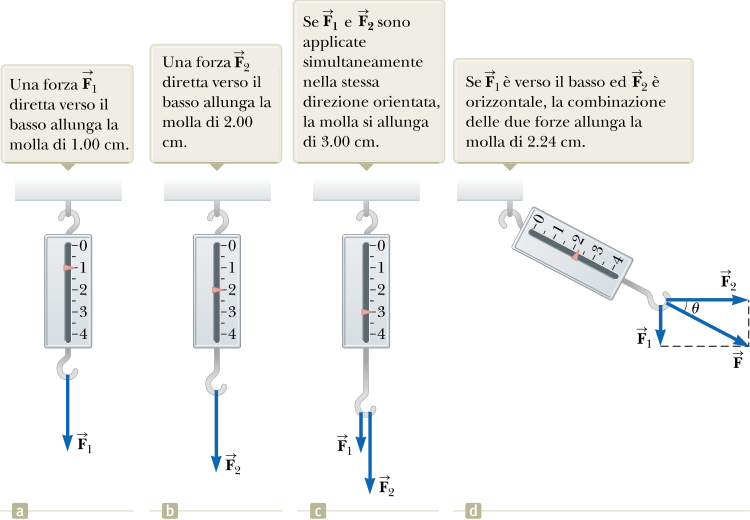
\includegraphics[scale=0.5]{natura_vettoriale_forze}
\end{figure*}
Come mostrato nella nel punto \emph{d} della figura, le due forze vengono applicate simultaneamente con $\vec{F}_1$ verticalmente verso
il basso e $\vec{F}_2$ orizzontalmente. In questo caso, l’indicatore indicherà \emph{2.24 cm}. La forza $\vec{F}$ che produce
la stessa lettura della somma dei due vettori $\vec{F}_1$ e $\vec{F}_2$. In altre parole, $\abs{\vec{F}_1} = \sqrt{F_1^2 + F_2^2} = 2.24$
unità e la sua direzione è $\theta = \tan^{-1} (-0.500) = -26.6$°

\paragraph{Dinamometro}
Il dinamometro è uno strumento di misura utilizzato in meccanica per determinare l'entità di una forza ad esso applicata.
Il meccanismo di misurazione utilizza il principio della legge di Hooke, per il quale la deformazione di un materiale elastico è direttamente proporzionale alla forza applicata al materiale stesso.

\newpage
\section{Prima legge di Newton - principio d'Inerzia}
La \textbf{prima legge di Newton} del moto, che viene spesso chiamata \textbf{legge d’inerzia},
definisce una particolare classe di sistemi di riferimento detti \textbf{sistemi inerziali}.
Questa legge può essere espressa nel seguente modo:
\begin{displayquote}
    \centering
    Se un corpo non interagisce con altri corpi, si può trovare un sistema di riferimento nel quale la sua accelerazione è nulla.
\end{displayquote}
Un tale sistema di riferimento viene chiamato \textbf{sistema di riferimento inerziale}.
Ogni sistema di riferimento che si muove a velocità costante rispetto ad un sistema di riferimento inerziale, è esso stesso un \emph{sistema inerziale}.

~\newline
Per i nostri scopi possiamo considerare anche la \emph{Terra come un sistema inerziale}. La Terra in realtà non è un sistema inerziale a causa del suo moto
orbitale intorno al Sole e del suo moto di rotazione intorno all’asse terrestre.
Queste accelerazioni hanno comunque valori piccoli rispetto a $g$ e possono spesso essere trascurate.

\noindent È possibile riformulare la \emph{prima legge di Newton} in un modo più pratico:
\begin{displayquote}
    \centering
    In assenza di forze esterne e se osservato da un sistema di riferimento inerziale, un corpo in quiete rimane in quiete ed un
    corpo in moto rimane in moto (con moto rettilineo uniforme).
\end{displayquote}

\paragraph{Inerzia} È possibile definire l'\emph{inerzia} come la \emph{tendenza di un corpo a non modificare il suo stato di moto}.

\subsection{Massa}
Quantitativamente il concetto di \emph{inerzia} viene quantificato dalla \textbf{massa}. La massa è la proprietà (scalare) di un corpo che misura
quanta resistenza un corpo offre al cambiamento di velocità. È una delle grandezze fondamentali.

L'unità di misura della massa \emph{m} è il \emph{kg}.

\paragraph{Rapporto massa-accelerazione}
Tra le due grandezze vi è un rapporto \emph{inversamente proporzionale}.

Si supponga di applicare una stessa forza $\vec{F}$ a due masse diverse $m_1$ e $m_2$, andando a misurare le accelerazioni $a_1$ e $a_2$ che la forza ha provocato.
Si verificherà la seguente relazione: $\frac{m_1}{m_2} \equiv \frac{a_1}{a_2}$

\newpage
\section{Seconda legge di Newton}
La \textbf{seconda legge di Newton} risponde alla domanda: che cosa succede ad un corpo se su di esso agiscono una o più forze?
\begin{itemize}
    \item L’accelerazione di un corpo è \emph{direttamente proporzionale} alla forza applicata su di esso: $\vec{F} \propto \vec{a}$
    \item L'intensità dell'accelerazione di un corpo è \emph{inversamente proporzionale} alla sua massa: $\abs{\vec{a}} \propto \tfrac{1}{m}$
\end{itemize}

Queste osservazioni sono sintetizzate dalla \emph{seconda legge di Newton}:
\begin{displayquote}
    \centering
    Misurata in un sistema di riferimento inerziale, l’accelerazione di un corpo è direttamente
    proporzionale alla forza risultante agente su di esso ed inversamente proporzionale alla sua massa:
    \begin{equation*}
        \vec{a} \propto \frac{\sum\vec{F}}{m}
    \end{equation*}
\end{displayquote}
Scegliendo la costante di proporzionalità pari a 1, è possibile scrivere la seguente equazione:
\begin{equation*}
    \sum\vec{F} = m\vec{a}
\end{equation*}
Questa equazione è un \emph{espressione vettoriale} e quindi è equivalente alle seguenti tre equazioni scalari, una per ogni componente:
\begin{align*}
    \sum F_x & = ma_x & \sum F_y & = ma_y & \sum F_z & = ma_z
\end{align*}

\paragraph{Unità di misura della forza}
L’unità di misura della forza nel SI, è il newton (N).
Una forza di $1 \; N$ è la forza che, se applicata ad un corpo di massa $1 \; kg$, produce una accelerazione di $1 \; m/s^2$.

Il newton può essere espresso in funzione delle unità fondametali di massa, lunghezza e tempo:
\begin{equation*}
    1 \; N \equiv 1 \; kg \cdot m/s^2
\end{equation*}
Per il sistema \emph{c.g.s.} esiste l'unità di misura ''dina''. 1 dina è la forza, che applicata a un corpo di massa 1 $g$, produce un accelerazione di 1 $cm/s^2$.

\subsection{La forza gravitazionale e il peso}
Un corpo in caduta libera (lasciato libero in prossimità della superficie terrestre) si muove con accelerazione costante pari a $g$ (9.81 $m/s^2$).
In base alla seconda legge di Newton, la forza che produce questa accelerazione, la forza di attrazione gravitazionale, equivale a $\vec{F_g} = mg$.

Il \emph{modulo} di questa forza viene chiamato \textbf{peso}: $F_g = mg$ (misurato in $N$).

\section{Terza legge di Newton}
«A un'azione è sempre opposta un'uguale reazione: ovvero, le azioni vicendevoli di due corpi l'uno sull'altro sono sempre uguali e dirette verso parti opposte.»

\begin{displayquote}
    \centering
    Per ogni forza, che un corpo $A$ esercita su un altro corpo $B$, ne esiste istantaneamente un'altra
    uguale in modulo e direzione, ma opposta in verso, causata dal corpo $B$ che agisce sul corpo $A$.
\end{displayquote}

~\newline
\underline{Esempio grafico:}

\begin{figure*}[h]
    \centering
    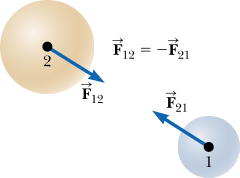
\includegraphics[scale=0.4]{terza_legge_newton}
\end{figure*}
\noindent Vediamo due corpi interagiscono che tra loro, la forza $\vec{F}_{12}$ esercitata dal corpo 1 sul corpo 2 è uguale in intensità ed è opposta
in verso alla forza $\vec{F}_{21}$ esercitata dal corpo 2 sul corpo 1:
\begin{equation*}
    \vec{F}_{12} = -\vec{F}_{21}
\end{equation*}

\paragraph{Diagramma di corpo libero}  Quando analizziamo un corpo soggetto a più forze, siamo interessati alla \textbf{forza risultante} 
su questo singolo corpo, che schematizzeremo come \emph{punto materiale}. Il diagramma di corpo libero, quindi, ci aiuta ad isolare solamente le forze che 
agiscono sul corpo ed eliminare dalla nostra analisi tutte le altre forze.

Nel \textbf{diagramma di corpo libero} è utilizzato il modello punto materiale per rappresentare il corpo come un punto e le forze che agiscono sul corpo sono applicate al punto.

\begin{figure*}[h]
    \centering
    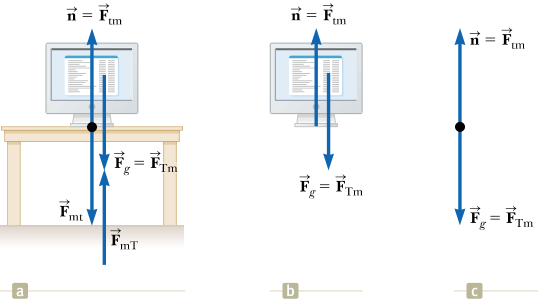
\includegraphics[scale=0.4]{diagramma_corpo_libero}
    \caption*{\small Il punto C dello schema rappresenta il \emph{diagramma di corpo libero}}
\end{figure*}

\section{Modelli di analisi}
\subsection{Punto materiale in equilibrio}
Se l’accelerazione di un corpo schematizzato come un punto materiale è nulla, il corpo verrà descritto con il modello \textbf{punto materiale in equilibrio}.
In questo schema, la forza risultante sul corpo è zero:
\begin{equation*}
    \sum \vec{F} = 0
\end{equation*}
\underline{Attenzione}: Anche un corpo che si muove a velocità costante può essere considerato \emph{in equilibrio}.

~\newline
\underline{Esempio: }
\begin{figure*}[h]
    \centering
    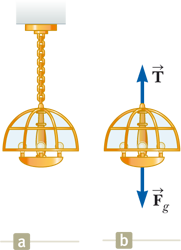
\includegraphics[scale=1]{lampada_in_equilibrio}
\end{figure*}
Le forze agenti sulla lampada sono la forza di gravità $\vec{F}_g$ verticale verso il basso e la forza di trazione $\vec{T}$ esercitata dalla catena verticalmente verso l'alto:
\begin{equation*}
    \sum F_y = 0 \;\; \rightarrow \;\; \sum F_y = T - F_g = 0 \;\; \rightarrow \;\; T = F_g
\end{equation*}
Si noti che, di nuovo, $\vec{T}$ e $\vec{F}_g$ \emph{non sono una coppia di forze di azione e reazione} perché esse sono applicate sullo stesso corpo, il lampadario.
La forza di reazione a $\vec{T}$  è applicata verso il basso dalla lampada alla catena.

\newpage
\subsection{Piano inclinato}
Esempio pratico:

\noindent Un’automobile di massa $m$ sta scivolando lungo una discesa ghiacciata inclinata di un angolo $\theta$, come mostrato in figura
\begin{figure*}[h]
    \centering
    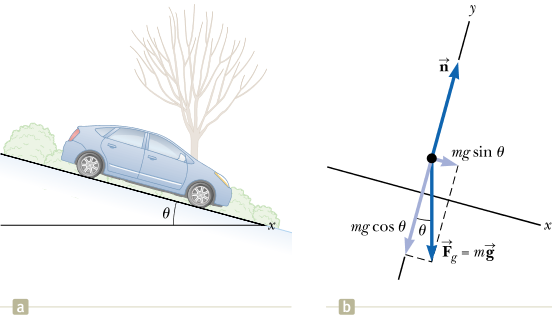
\includegraphics[scale=0.45]{piano_inclinato} ~~
    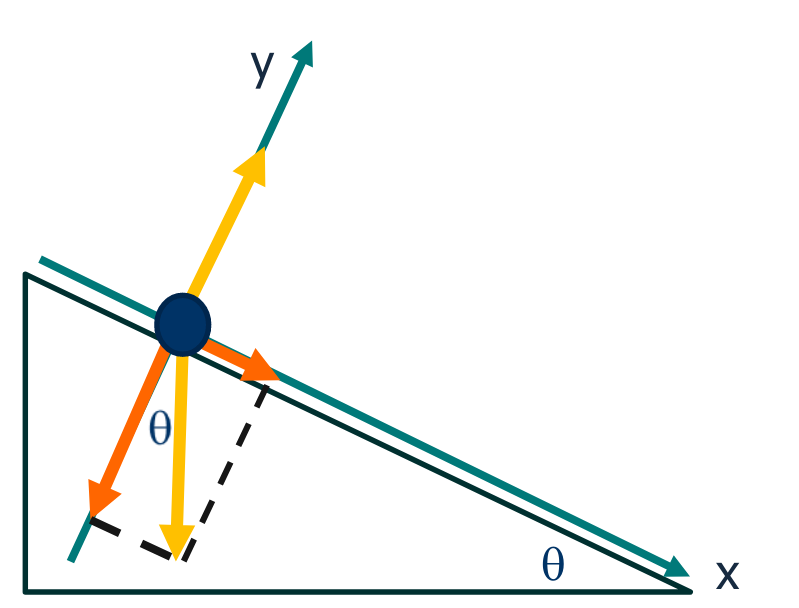
\includegraphics[scale=0.2]{piano_inclinato_forze}
\end{figure*}

\noindent Le forze in gioco sono:
\begin{itemize}
    \item \textbf{Forza peso} $\vec{F}_g = m\vec{g}$, sempre verticale verso il basso, divisa nelle sue componenti $x$ e $y$
    \begin{itemize}
        \item $\vec{F}_{gx} = mg \sin{\theta} = ma_x = \sum F_x$
        \item $\vec{F}_{gy} = mg \cos{\theta}$
    \end{itemize}
    \item \textbf{Reazione vincolare} $\vec{n}$, perpenticolare al piano
\end{itemize}
Sull'asse y non è presente accelerazione: $\sum F_y = n - mg \cos{\theta} = 0$ \newline
L'accelerazione in x quindi vale $a_x = g \sin{\theta}$ \newline
La reazione vincolare è pari a $n = mg \cos{\theta}$

\section{Forze di attrito}
Quando un corpo è in moto o su di una superficie o in un mezzo viscoso, come l’aria o l’acqua, 
nasce una \emph{resistenza al moto} a causa delle interazioni tra il corpo ed il mezzo che lo circonda. Questa resistenza prende il nome di \textbf{forza di attrito}.
\begin{figure*}[h]
    \centering
    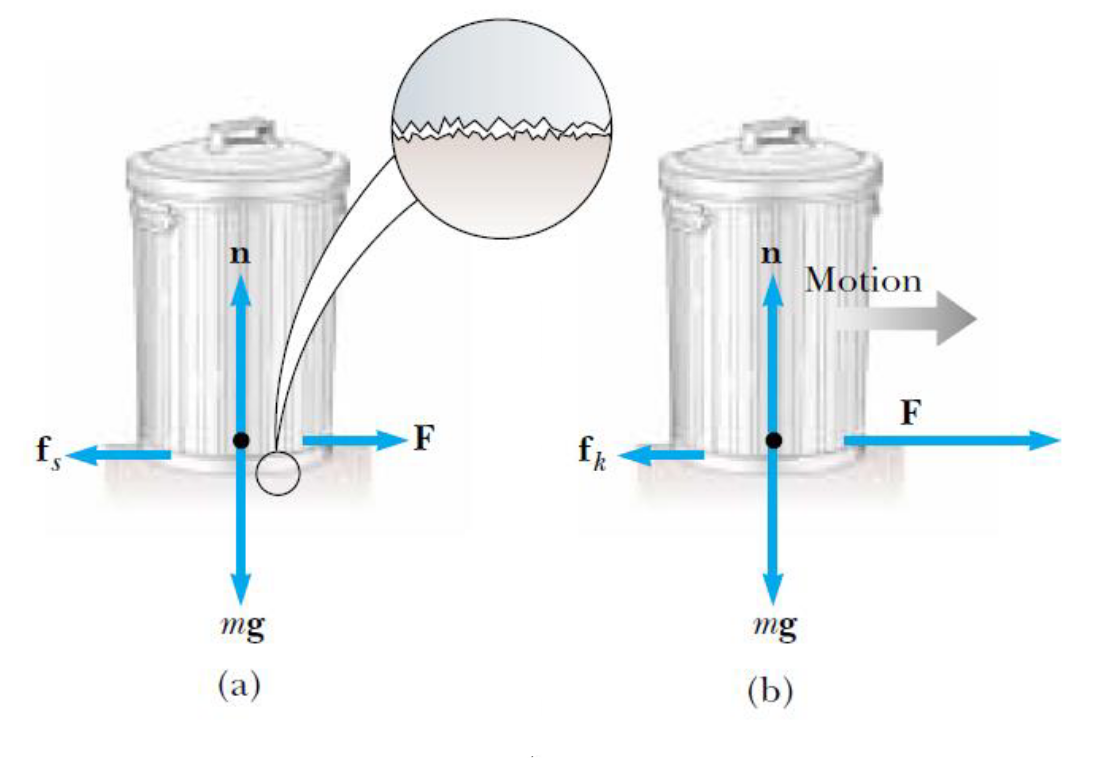
\includegraphics[scale=0.23]{attrito_bidone}
\end{figure*}

\paragraph{Attrito statico}
Se applichiamo a un'oggetto una forza $\vec{F}$ esterna orizzontale verso destra e se la forza $\vec{F}$ che applichiamo è piccola, l'oggetto rimarrà fermo.

La forza che agisce sull'oggetto e che contrasta $\vec{F}$ impedendogli di muoversi verso sinistra, prende il nome di forza di \textbf{attrito statico} $\vec{f}_s$.

Fino a quando l'oggetto rimane fermo, si ha $\vec{f}_s = \vec{F}$. Quindi se $\vec{F}$ aumenta, aumenterà anche $\vec{f}_s$. In ugual modo, se $\vec{F}$ diminuisce, diminuirà anche $\vec{f}_s$ .

L’intensità della forza di attrito statico tra due superfici qualunque a contatto tra loro può assumere i valori
\begin{equation*}
    f_s \le \mu_s n
\end{equation*}
dove la costante adimensionale $\mu_s$ è chiamata \textbf{coefficiente di attrito statico}.

\paragraph{Attrito dinamico}
Aumentando il valore di $\vec{F}$, l'oggetto arriverà sul punto di iniziare a muoversi, $\vec{f}_s$ raggiunge il suo valore massimo, $\vec{f}_{s,max}$.

Quando F supera il valore $\vec{f}_{s,max}$, il bidone inizierà a muoversi e, quindi, ad accelerare verso destra. La forza di attrito su di un corpo in movimento prende il nome di \textbf{forza di attrito dinamico} $\vec{f}_k$.
La forza risultante è $\vec{F} - \vec{f}_k > 0$ (moto).

Quando il bidone è in moto, il valore della forza di attrito dinamico che agisce sul corpo è \underline{minore} di $\vec{f}_{s,max}$. 

L’intensità della forza di attrito dinamico tra due superfici qualunque a contatto tra loro è
\begin{equation*}
    f_k = \mu_k n
\end{equation*}
dove la costante adimensionale $\mu_k$ è chiamata \textbf{coefficiente di attrito dinamico}.

\begin{figure*}[h]
    \centering
    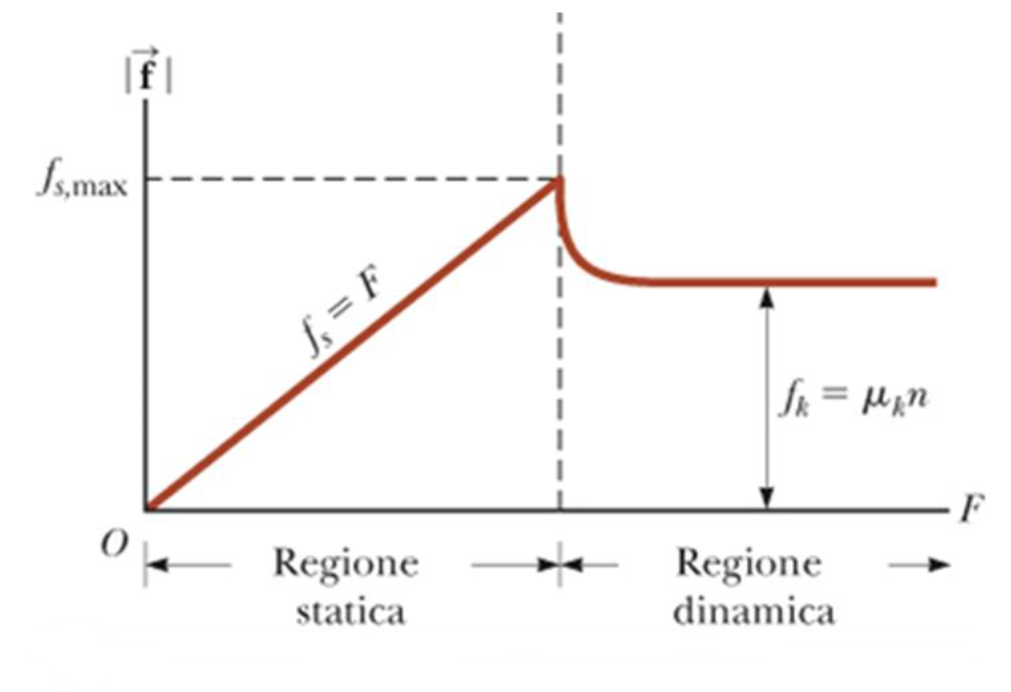
\includegraphics[scale=0.3]{forze_attrito_grafico}
\end{figure*}
\noindent Sperimentalmente, sia $\vec{f}_k$ che $\vec{f}_{s,max}$ hanno moduli proporzionali al modulo di $n$.

\newpage
\section{Altre applicazioni delle leggi di Newton}

\subsection{Estensione del Moto Circolare Uniforme}
Nel moto circolare uniforme il punto materiale si muove con velocità in modulo $v$ costante lungo una traiettoria circolare di raggio $r$.
Il punto materiale si muove con \textbf{accelerazione centripeta} di modulo
\begin{equation*}
    a_c = \frac{v^2}{r}
\end{equation*}
L'accelerazione è diretta verso il \emph{centro} ed è perpendicolare a $v$. Per la seconda legge di Newton, la forza risultante che produce l'accelerazione centripeta
può essere messa in relazione con l'accelerazione come segue:
\begin{equation*}
    \sum F = ma_c = m \frac{v^2}{r}
\end{equation*}
Una forza che produce un’accelerazione centripeta deve agire nella direzione che punta al \textbf{centro} del percorso circolare e provoca una variazione della direzione del vettore velocità.

\subsection{Moto Circolare non Uniforme}
se un punto materiale si muove con velocità di modulo variabile su un percorso circolare, ci deve essere, oltre alla componente radiale della accelerazione, una componente tangenziale di modulo $\abs{\tfrac{dv}{dt}}$. Quindi, anche la forza agente sulla particella deve avere una componente tangenziale ed una radiale.
\begin{figure*}[h]
    \centering
    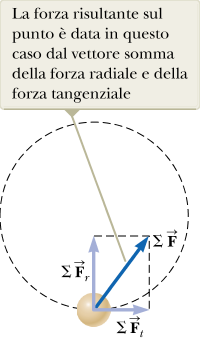
\includegraphics[scale=0.4]{newton_moto_circolare_non_uniforme.png}
\end{figure*}

\noindent L'accelerazione risultante è:
\begin{equation*}
    \vec{a} = \vec{a_r} + \vec{a_t}
\end{equation*}
E di conseguenza la forza risultante esercitata sulla particella è:
\begin{equation*}
    \sum \vec{F} = \sum \vec{F_r} + \sum \vec{F_t}
\end{equation*}
Il vettore $\sum \vec{F_r}$ è diretto verso il centro della circonferenza ed è responsabile dell’accelerazione centripeta. 
Il vettore $\sum \vec{F_t}$ tangente alla circonferenza è responsabile della accelerazione tangenziale, che rappresenta una variazione nel tempo del modulo 
della velocità del punto materiale.

\section{Moto in presenza di forze frenanti}
Consideriamo ora l'interazione tra il corpo in movimento e il mezzo nel quale esso si muove, che può essere un liquido o un gas. Il mezzo esercita una \textbf{forza frenante} $\vec{R}$ sul corpo che lo sta attraversando.
L’intensità di $\vec{R}$ dipende dal \emph{modulo} della velocità del corpo, mentre il verso di $\vec{R}$ è sempre \emph{opposto alla direzione di moto} del corpo relativamente al mezzo attraversato.

\subsection{Forza frenante proporzionale alla velocità del corpo}
Se facciamo l’ipotesi che la forza frenante che agisce su un corpo in moto in un liquido o in un gas sia proporzionale alla velocità del corpo, allora la forza frenante può essere espressa come
\begin{equation*}
    R = -b\vec{v}
\end{equation*}
dove $b$ è una \textbf{costante} il cui valore dipende dalle \emph{proprietà del mezzo}, dalla forma e dalle dimensioni del corpo, e $\vec{v}$ è la velocità del corpo rispetto al mezzo.

~\newline
\underline{Esempio}: Sfera di massa $m$ lasciata cadere in un liquido.
\begin{figure*}[h]
    \centering
    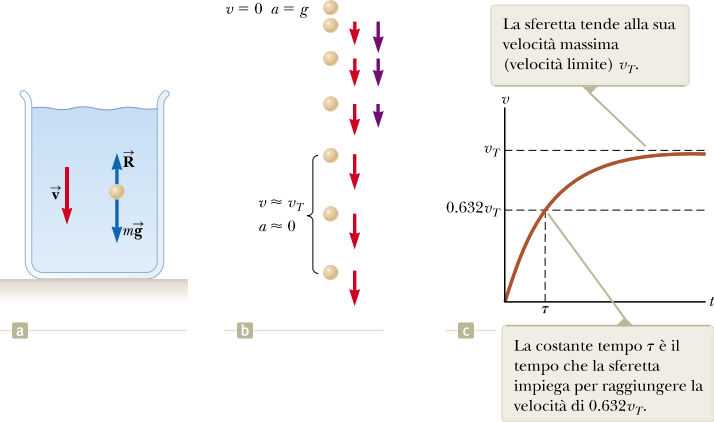
\includegraphics[scale=0.4]{sfera_fluido.png}
\end{figure*}

\noindent La sommatoria delle forze che agiscono è 
\begin{equation*}
    \sum F_y = mg - bv = ma
\end{equation*}
Al crescere del tempo cresce la velocità e di conseguenza cresce anche l'intensità della forza frenante R. Si arriverà ad un punto in cui $\abs{R} = \abs{F_p}$
In queste condizioni l'accelerazione diventerà nulla $a=0$ e la velocità tenderà alla \textbf{velocità limite} $v_T$.
\begin{align*}
    mg - bv_T = 0 \;\; \rightarrow \;\; v_T = \frac{mg}{b}
\end{align*}

~\newline
La velocità in funzione del tempo si ricava con:
\begin{equation*}
    v = v_T(1-e^{-t/\tau})
\end{equation*}
dove la \textbf{costante di tempo} $\tau = \tfrac{m}{b}$ corrisponde all’intervallo di tempo nel quale la sferetta partendo da ferma raggiunge il $63.2\%$ del valore della sua $v_T$.

\chapter{Energia}

\section{Energia di un sistema}
\subsection{Lavoro compiuto da una forza costante}
In fisica, il \textbf{lavoro} è l'\emph{energia scambiata tra due sistemi} quando avviene uno spostamento attraverso l'\emph{azione di una forza}, o una risultante di forze, che ha una componente non nulla nella direzione dello spostamento. 
Pertanto, ha le dimensioni di una forza applicata lungo una determinata distanza. 

Il lavoro W compiuto su un sistema da un agente che esercita su di esso una forza costante è uguale al prodotto tra il \textbf{modulo $F$ della forza}, 
il \textbf{modulo $\Delta r$ dello spostamento} del punto di applicazione della forza e {\boldmath$\cos{\theta}$}, dove $\theta$ è l’angolo tra il vettore forza e il vettore spostamento:
\begin{equation*}
    W \equiv F \Delta r \cos{\theta}
\end{equation*}
L'unità di misura del \textbf{lavoro} è: $N \cdot m = kg \cdot m^2/s^2 = J \; \text{(joule)}$.

~\newline \underline{Alcune osservazioni}:
\begin{itemize}
    \item Una forza compie un lavoro nullo su un corpo se esso non viene spostato. Infatti, se $\Delta r$ = 0, l’Equazione fornisce $W$ = 0.
    \item Il lavoro compiuto da una forza su un corpo in movimento è zero quando la forza applicata è perpendicolare allo spostamento del suo punto di applicazione. Infatti, se $\theta = 90^\circ$ allora $W = 0$ poiché $\cos{90^\circ} = 0$.
    \item Il lavoro compiuto dalla forza applicata su un sistema è positivo quando la proiezione di $\vec{F}$ lungo la direzione di $\Delta \vec{r}$ ha lo stesso verso dello spostamento.
    Quando la proiezione di $\vec{F}$ lungo la direzione di $\Delta \vec{r}$ ha verso opposto a quello dello spostamento, $W$ è negativo.
    \item Una considerazione importante nell’approccio ai problemi consiste nel pensare al lavoro come \textbf{trasferimento di energia}. Se $W$ è il lavoro compiuto su un sistema 
    e $W$ è positivo, dell’energia viene trasferita \emph{al sistema}; se $W$ è negativo, dell’energia è trasferita \emph{dal sistema}.
\end{itemize}

\subsection{Prodotto scalare tra due vettori}
Per tener conto del modo in cui i vettori forza e spostamento sono combinati, è utile introdurre un appropriato strumento matematico chiamato \textbf{prodotto scalare tra due vettori}. 
Il prodotto scalare tra i vettori $\vec{A}$ e $\vec{B}$ viene indicato con l’espressione $\vec{A}\cdot\vec{B}$.

Il prodotto scalare tra due vettori $\vec{A}$ e $\vec{B}$ è una quantità scalare uguale al prodotto dei moduli dei due vettori per il coseno dell’angolo $\theta$ compreso tra di essi:
\begin{equation*}
    \vec{A} \cdot \vec{B} = AB\cos{\theta}
\end{equation*}
Confrontando tale definizione con l'equazione , possiamo esprimere l’equazione del \textbf{lavoro} sotto forma di un prodotto scalare:
\begin{equation*}
    W = F \cdot \Delta r \cdot \cos{\theta} = \vec{F} \cdot \Delta \vec{r}
\end{equation*}

\section{Lavoro di una forza variabile}
Consideriamo un punto materiale che si sposta lungo l’asse x sotto l’azione di una \emph{forza che varia con la posizione}. In tale situazione, non è possibile utilizzare l'equazione vista in
precedenza per calcolare il lavoro fatto dalla forza in quanto tale relazione si applica solo se il vettore $\vec{F}$ rimane costante in modulo, direzione e verso.

\begin{wrapfigure}{r}{0.20\textwidth}
    \centering
    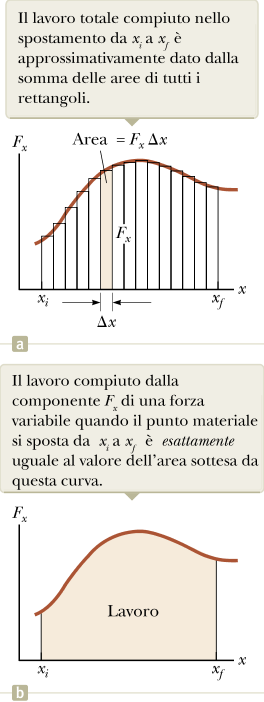
\includegraphics[width=0.20\textwidth]{lavoro_forza_variabile.png}
\end{wrapfigure}
Possiamo suddividere l'intervallo in tanti piccoli intervalli di spostamento $\Delta x$ e assumere che la forza in ogni intervallo valga un dato $F_x$. 
Il lavoro complessivo sarà quindi approssimato con la sommatoria
del lavoro di ogni intervallo:
\begin{equation*}
    W \approx \sum_{x_i}^{x_f} F_x \Delta x
\end{equation*}
Per migliorare questa approssimazione valutiamo il limite per $\Delta x \to 0$:
\begin{align*}
    \lim_{\Delta x \to 0} \sum_{x_i}^{x_f} F_x \Delta x &= \int_{x_i}^{x_f} F_x \; dx & W&= \int_{x_i}^{x_f} F_x \; dx
\end{align*}
Se sul corpo agiscono più forze (nella direzione x):
\begin{equation*}
    \sum W = W_{est} = \int_{x_i}^{x_f} \big(\sum F_x \big) \; dx
\end{equation*}
Se una forza risultante variabile in modulo e direzione agisce sul corpo:
\begin{equation*}
    \sum W = W_{est} = \int_{x_i}^{x_f} \big(\sum \vec{F} \big) \cdot d \; \vec{r}
\end{equation*}


\subsection{Lavoro compiuto da una molla}
Lo schema di un sistema fisico molto comune nel quale la forza varia in funzione della posizione è mostrato in Figura. Il sistema è un blocco che giace su una superficie orizzontale senza attrito, collegato ad una molla.
se la molla viene allungata o compressa di un piccolo tratto rispetto alla sua lunghezza di riposo (equilibrio), essa esercita sul blocco una forza che matematicamente può essere espressa nella forma
\begin{align*}
    F_s &= -kx & &\text{\textbf{Legge di Hooke}} 
\end{align*}
dove $x$ indica la posizione del blocco rispetto alla sua posizione di equilibrio $(x = 0)$ e $k$ è una costante positiva chiamata \textbf{costante elastica} della molla.

\newpage
\begin{figure*}[h]
    \centering
    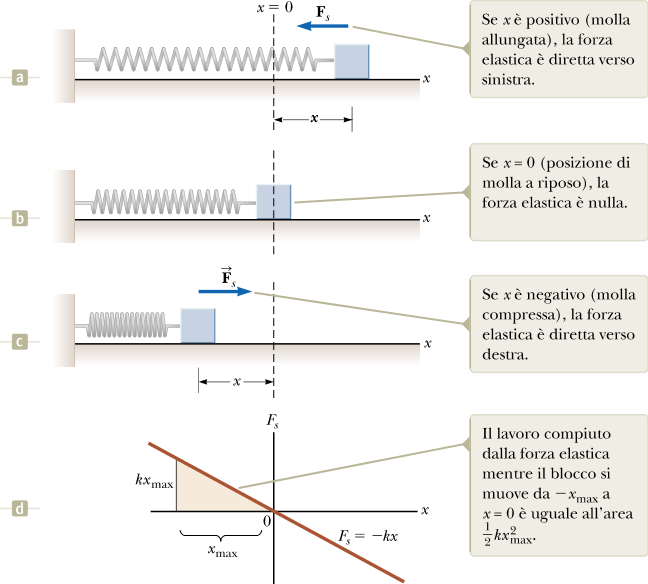
\includegraphics[scale=0.4]{lavoro_molla.png}
\end{figure*}
Il valore di k dà una misura della rigidità della molla. Molle “rigide” hanno grandi valori di k, mentre per molle “morbide” i valori di k sono piccoli. L'unità di misura di $k$ corrisponde a $N/m$.
Il lavoro della forza elastica sarà
\begin{equation*}
    W_s = \int_{x_i}^{x_f}F_s \;dx
\end{equation*}
Ipotizzando di partire dal punto di massima compressione della molla ($-x_{max}$) ed arrivare al punto $x=0$
\begin{equation*}
    W_s = \int_{x_i}^{x_f}F_s \; dx = \int_{-x_{max}}^{0} (-kx) \; dx = \tfrac{1}{2}kx^2_{max}
\end{equation*}
Per uno spostamento arbitrario da $x_i$ a $x_f$:
\begin{equation*}
    W_s = \int_{x_i}^{x_f}F_s \; dx = \tfrac{1}{2} kx_i^2 - \tfrac{1}{2}kx_f^2
\end{equation*}
Da notare che, per qualunque spostamento in cui punto iniziale e punto finale coincidono, il lavoro è nullo.

Consideriamo ora il lavoro compiuto sul blocco da un agente esterno che applica una forza sul blocco mentre questo si sposta molto lentamente da $xi = -x_{max}$ a $x_f = 0$.
Possiamo calcolare questo lavoro osservando che per ogni valore della posizione, la forza applicata $\vec{F}_{app}$ è uguale in modulo e opposta in verso alla forza elastica $\vec{F}_s$, cosicché
\begin{gather*}
    F_{app} = -(-kx) = kx \\ 
    W_{F_{app}} = \int_{0}^{x_{max}} F_{app} \; dx = \int_{0}^{x_{max}} kx \; dx = \tfrac{1}{2}kx^2_{max}
\end{gather*}
Per uno spostamento arbitrario del blocco, il lavoro compiuto sul sistema dall'agente esterno è dato da 
\begin{equation*}
    W_{F_{app}} = \int_{x_i}^{x_f} F_{app} \; dx = \int_{x_i}^{x_f} kx \; dx = \tfrac{1}{2}kx_f^2 - \tfrac{1}{2} kx_i^2
\end{equation*}

\section{Energia Cinetica}
Una possibile \emph{conseguenza del lavoro} compiuto su un sistema è la \emph{variazione della sua velocità}. L'\textbf{energia cinetica} è l'energia che un corpo possiede a causa del proprio movimento.

\begin{figure*}[h]
    \centering
    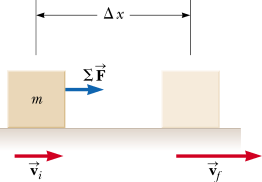
\includegraphics[scale=0.4]{energia_cinetica_schema.png}
\end{figure*}
La figura mostra un blocco di massa $m$ che si muove verso destra sotto l’azione di una forza risultante $\sum \vec{F}$ verso destra. Dalla seconda legge di Newton sappiamo che il blocco si muove con un’accelerazione $\vec{a}$.
Essendo la forza costante, il moto è \emph{uniformemente accelerato}. Per cui vale la relazione
\begin{align*}
    v_f^2-v_i^2 &= 2a(x_f-x_i) \\
    &= 2\frac{F}{m}(x_f-x_i)
\end{align*}

\end{document}
